% Chapter 2

\chapter{Hardware} % Main chapter title

\label{hardware} % For referencing the chapter elsewhere, use \ref{Chapter1} 

\lhead{Chapter 2. \emph{Hardware}} % This is for the header on each page - perhaps a shortened title

%----------------------------------------------------------------------------------------

\section{Inverter Systems Overview}

Power inverters are used for converting the DC power output of photovoltaic (PV) panels, batteries, or other DC sources into the AC power used in power grids worldwide. Our microinverter has three main power conversion stages, namely the DC/DC boost, H-bridge, and output filter. We will refer to the combination of H-Bridge and switching scheme frequenctyl throughout this work simply as `the inverter.'  What we refer to as `the inverter' consists of an H-Bridge and transistor driver hardware that creates the pseudo-sinusoidal wave from the high voltage DC output of the boost. The inverter is of central concern in this work, and in particular, the pseudo-sinusoidal waveforms that result from our control scheme - these were mentioned briefly in Sections \ref{squareApproach}, \ref{pwmApproach}, and \ref{hybridApproach}, but will be discussed in detail in Chapter \ref{Chapter5}, Section \ref{fourier} - however, an inverter cannot operate in a vacuum. Therefore, we must first offer some background on the complete hardware system supporting the operation of the inverter system as a whole shown in Figure~\ref{solarBlock}. The following subsections will provide a detailed account of the role that each component part plays in the system.

\subsection{Logic Power Supply}

Logic power is sourced from the solar panel via a buck converter IC; a buck converter is an efficient means of converting high DC voltages into smaller DC voltages without generating an excess of waste heat, as is typical with LDO regulators. The buck converter steps input voltage down from approximately $35-45V$ to $12V$. To combat the relatively high harmonic content of the buck converter and the nefarious effect it would ave on our sensitive analog circuitry, we use LDO's to produce stable, and much cleaner, $5v$ and $3.3V$ rails for the supporting cast of hardware on our inverter - namely, the microcontroller, FET gate drivers, and op-amp sensing circuits. 

\todo[inline]{Ben wrote this}
A logic power supply is required for the inverter board to run the microcontroller, driver circuits, and peripheral sensor network. Three different voltage rails were needed at $12V$, $5V$ and $3.3V$. The input from the solar panel was utilized to create these different power rails through a small connection circuit. Efficiency of this type of system is considered crucial, so cascaded switching DC/DC buck converters were used to create the $12V$ and $5V$ rails. A fast responding low-dropout linear regulator created the final $3.3V$ from the $5V$ rail. The circuit schematic for the logic power supply is shown in Figure~\ref{logic power fig}.

A variety of features were added to this front input interface for system protection and functionality. There are two options for sourcing power to the inverter board: banana jack connections for solar input and a DC barrel jack plug for testing input. These two circuits are configured so that only the barrel jack will source power if both happened connected and energized at the same time. Two switches are included for toggling the DC jack input and for switching conversion power into the main system. A ten amp blow fuse is included in series with the input to the inverter to prevent damaging short circuit conditions. A green LED on the $3.3V$ rail turns on to show the system is receiving power.\todo[inline]{this whole paragraph is shot! Redo}

\subsection{Boost Converter}
The boost converter steps up the relatively low voltage sourced from one or two PV panels while implementing maximum power point tracking (MPPT) to keep the system operating near peak efficiency - this stage is critical for maximizing return on investment (ROI) in the face of the non-linear characteristics of the PV panel. The boost circuit trades current for voltage, much like a transformer, by harvesting the inductive kick of an inductor hooked up to a switch. By the fundamental relationship
\begin{equation}
V=L\frac{\delta i}{\delta t}
\end{equation}
 we see that the faster we can change current through the inductor, the larger voltage spike we can capture. This `capture' is done with a diode and capacitor circuit.

\todo[inline]{Ben wrote this}
A standard PV microinverter contains two principle energy conversion stages with a DC/DC module and DC/AC module. This section highlights the hardware design process of a DC/DC boost converter for solar microinverter implementations. The boost circuit includes many elements and considerations of the final inverter system including power switching hardware and sensor circuits. The boost stage designed is essential for photovoltaics since it allows consistent maximum power sourcing from the panel. Solar panels have nonlinear relationships between output voltage and current. The maximum power product of the electrical values will vary depending on light intensity levels, loading, and temperature. A microcontroller unit (MCU) is used with this boost converter for create a feedback control scheme called a maximum power point tracker (MPPT). A versatile DC/DC boost stage is needed for microinverters since it can dynamically vary power switching based on the MPPT to compensate for the wide range of potential solar panel voltages. This converter topology utilizes a discrete MOSFET for switching since microcontroller interfacing is required. Traditional boost converter integrated circuits (ICs) do not satisfy the MPPT control needs or power requirements needed for this type of system.  \todo[inline]{this whole paragraph needs work. Think about our audience being pretty smart people, try to use some economy with your words}

A generic boost converter circuit shown in Figure~\ref{Figure 3}. Operation of a boost converter has two distinct phases depending on the switch mode of the power MOSFET. The gate of the MOSFET is sent different logic values at specific duty cycles through PWM. When the drive circuit outputs logic high in Figure 3 \todo[inline]{no-no}, the drain to source path will conduct in the saturation region. This provides a path to ground for the current flowing through the inductor and reverse biases the clamp diode. Over time energy is built up in the magnetic field of the inductor coil from this solar panel sourced current. Then logic low is sent to the MOSFET to shut it down. Considering the sudden change in current flow, a large voltage kickback occurs across the inductor and forward biases the diode. Current now can flow to charge the output capacitor and feed the load.

\begin{figure}
\centering
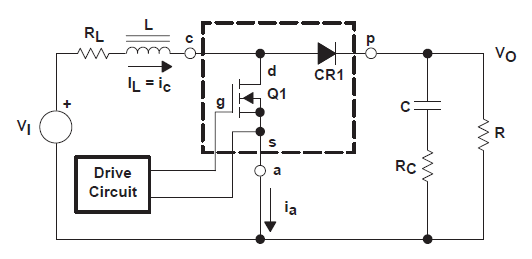
\includegraphics[width = 3.5in]{Generic_Boost_Converter.PNG}
\caption{Traditional Boost Converter Circuit}
\label{Figure 3}
\end{figure}

When the MOSFET is conducting, the output capacitor provides power to the load until it receives new charge during the second period. Due to the switching characteristics and inductor physics, a large ripple current flows through the inductor. An important design constraint it to make sure the inductor current always remains greater than zero such that continuous conduction mode (CCM) is maintained. CCM ensures a desired voltage transfer function for gain in this design. Additionally, there are some parasitic elements included in the circuit that contribute to power loss. These undesired effects include the DC resistance of the inductor windings and the equivalent series resistance of the capacitor.  
The electrical specifications of this boost converter are listed in Table~\ref{Table 1}. \\ 
\todo[inline]{the rest of this section needs work too}

\begin{table}
\centering
\begin{tabular}{|c|c|}
\hline
 Parameter & Value \\
 \hline
 $ V_{in} = V_{panel}$ & 0V to 40V DC \\
 \hline
 $ I_{in}$ & 5.47A DC max \\
 \hline
 $ V_{out}=V_{load} $ & 169.73V Min to 200V max \\
 \hline
 $ I_{out} $ & 1.18A DC max \\
 \hline
 $ P_{rated} $ & 200W \\
 \hline
 $ f_{switching} $ & 50 kHz \\
 \hline
\end{tabular}
\caption{Electrical Specifications for Boost Converter}
\label{Table 1}
\end{table}

The Sharp solar panels, utilized in this design as an input power source, \todo[inline]{the fuck else would we use them for?} will have varying voltage and current output capabilities depending on lighting conditions. Maximum output power for the 170W panels occurs at $V_{panel}=34.8V$ and  $I_{panel} = 4.9A$. An input voltage range will be selected to define a sourcing range with usable power output considering the panels highly nonlinear relationship regarding I vs V shown \todo[inline]{I don't understand what youre trying to say here} in Figure~\ref{Figure 4} \todo[inline]{I'm gonna lose my shit if this doesnt get fixed. we need sensible labels for everything}. Output voltage is defined based on the minimum value needed for the 120Vrms/0.707 = 169.73V \todo[inline]{this needs to be written in math mode} peak value needed for the DC/AC inverter stage input. Maximum power of 200W is an upper limit buffer set for this design considering the solar panel approach with microinverter topology. Switching frequency is set at 50 kHz based on recommended ranges and to compare to the TI Solar Explorer Development Board also used in this project.\cite{SharpPanel}

\begin{figure}
\centering
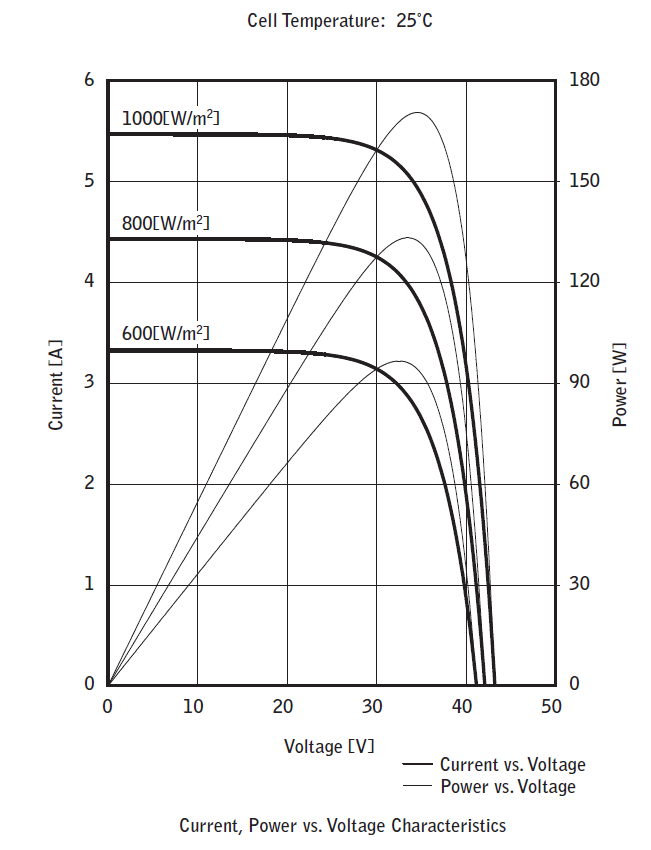
\includegraphics[width = 3.5in]{solar_v_vs_i.PNG}
\caption{Solar Panel IV Characteristics}
\label{Figure 4}
\end{figure}
\todo[inline]{you need to cite this figure, and all others you used}

The process of designing the boost circuit hardware involved a review of application notes, and in running PSPICE simulations. PSPICE computer software \todo[inline]{computer software? are you 70?} produced by Cadence\textbackslash{}OrCAD was used to simulate the boost converter. The max power voltage \todo[inline]{power voltage?} of the PV panels was selected for primary simulation testing. Calculations were performed to best select power components for operations of the boost converter at high power values \todo[inline]{how does power affect component values apart from size/rating?}. These design steps considered power dissipation thermal limits, critical inductance, and critical capacitance. The PSPICE circuit encapsulating the entire boost converter design is shown in Figure~\ref{boostCrct}.

\begin{figure}
\centering
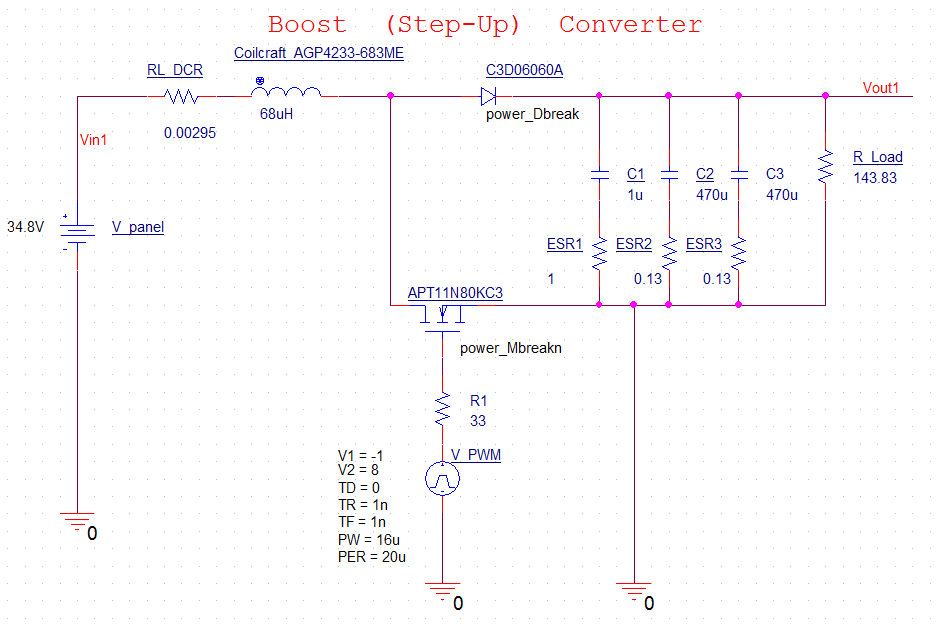
\includegraphics[width = 3.5in]{Boost_Circuit.PNG}
\caption{PSPICE Boost Converter Simulation}
\label{boostCrct}
\end{figure}

The operation of the boost converter in PSPICE required a switching signal to control the power MOSFET. Implementation of the converter will utilize C2000 MCU logic signals and Silicon Labs gate driver circuits for MOSFET switching. This simulation uses a variable duty cycle pulse source \todo[inline]{pulse source? just say duty cycle} for continuous switching at the set frequency. This configuration is currently being run open-loop, but will include a compensation feedback control circuit to maintain stable output voltage in the final design. The solar panel 34.8V input at max power required a duty cycle set at 80.13\% for the PWM switching signal to achieve 169.73Vdc \todo[inline]{needs to be math mode} out. A load of 143.83$\Omega$ \todo[inline]{put numbers in math mode}was connected at the output to simulate max power current draw and realize the 200W capability of the system. Real output power will be less in practice due to additional inefficiencies, panel operating conditions, and sourcing configuration capabilities. The output power, current and voltage as the boost converter approaching\todo[inline]{read this out loud} steady-state conditions from start-up are shown in the simulation plot of Figure~\ref{Figure B}. \todo[inline]{simulation plot? you don't plot a simulation, you plt its results}

\begin{figure}
\centering
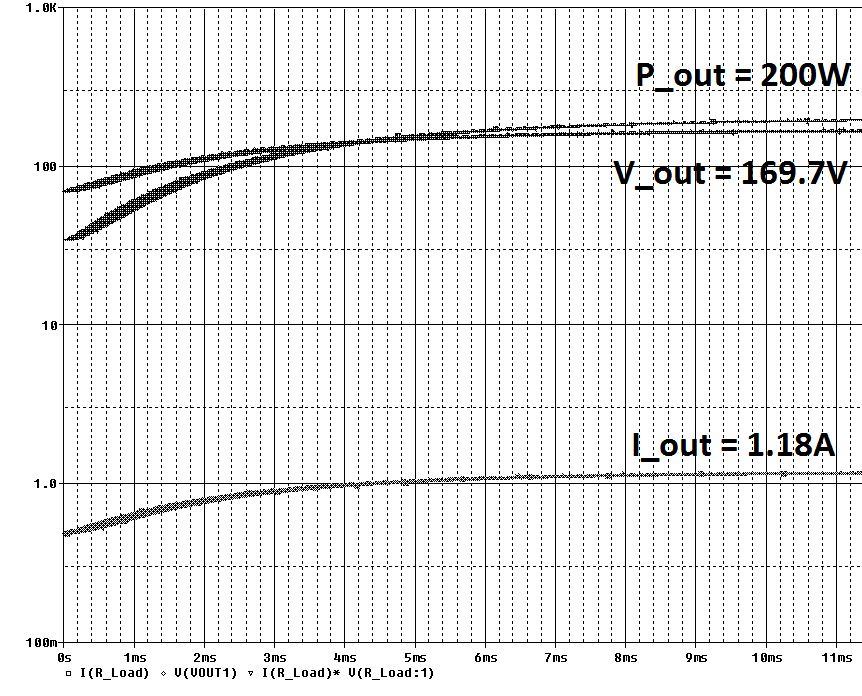
\includegraphics[width = 3.5in]{Boost_Power.png}
\caption{Boost Converter Approaching Steady State}
\label{Figure B}
\end{figure}

This boost converter was designed to operate in continuous condition mode (CCM). Ensuring this condition meant that the inductor current will \todo[inline]{you say ensuring this condition meant... then you give a definition of what CCM is. Say what CCM is, then say how you prevent it} never fall to zero and the panels are always sourcing current. This was achieved by selecting an inductor value above the calculated critical inductance and making sure it has appropriate current handling capabilities. Figure~\ref{Figure c} shows the rippled inductor current in CCM and the MOSFET switching signal that creates these dynamic effects in the boost converter. 

\begin{figure}
\centering
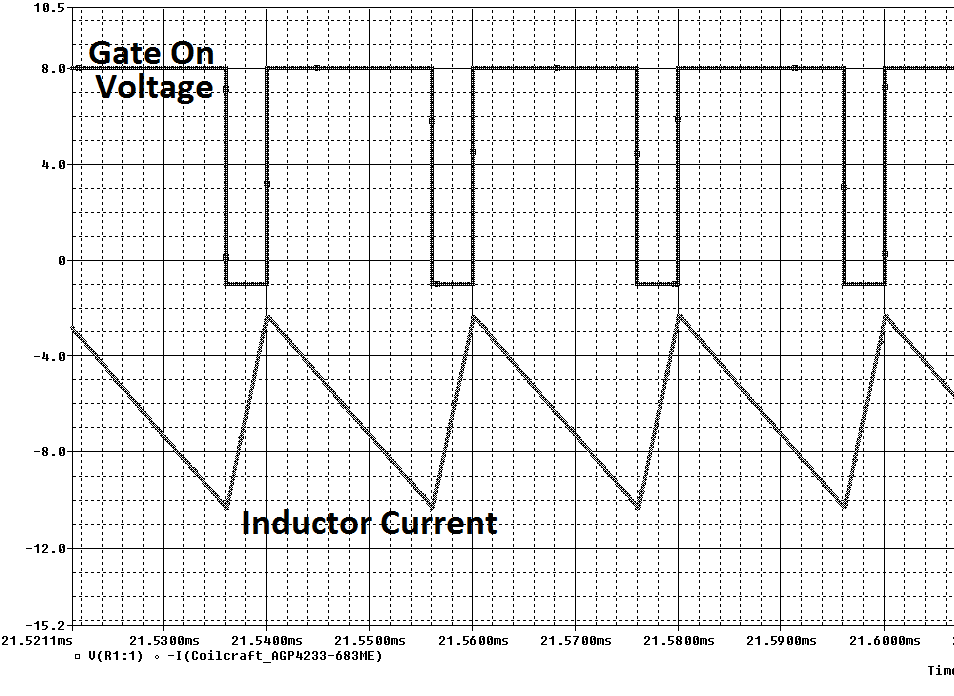
\includegraphics[width = 3.5in]{Boost_Inductor_Current_Steady_State.png}
\caption{Switching Signal and Inductor Current}
\label{Figure c}
\end{figure}

Another factor influencing the switching of the MOSFET is the maximum power-point tracking (MPPT) algorithm implemented by the microcontroller. This works to vary the input impedance of the converter as seen by the panel to optimize power output at 34.8V. \todo[inline]{I dont know that its appropriate to talk about MPPT here, you dont explain how it affects switching, just that it will. Let's make a section for MPPT in software}This method uses feedback control based on the voltage and currents measured by the ADC to perturb and observe the boost condition. Since the solar panel voltage can vary, the simulation circuit was run at the minimum 20V to check that the power output voltage could be maintained. The simulation results confirm this with $V_{out}=169.73V$, $V_{panel,in}=20V$, and a new duty cycle set at 89.25\%. \todo[inline]{more evidence that MPPT is out of place here - if we don't know what the MPPT is, how are we gonna give a fixed duty cycle? You need to make it clear that the hardware alons is open loop, only with software does it become a living thing}

Ratings on voltages and currents concerning components were determined through worst case calculations.\cite{kwasinski} 
\begin{equation}
I_L = I_{diode} = I_{drain} = \frac{2}{\sqrt[2]{3}}I_{in,rms} 
\end{equation}
\begin{equation}
 V_{cap} = V_{out} = 1.5V_{out,typ} = 2(169.73V) = 254.6V 
\end{equation}
\begin{equation}
 V_{diode} = V_{DS,FET} = 2(169.73V) =339.46V  
\end{equation}
\begin{equation}
I_{cap} = I_{out,rms} = 1.18A 
\end{equation}
The clamp diode was selected to be a Silicon Carbide (SiC) schottky type \todo[inline]{remove `type', this is obvious, requires a rewrite of this sentence} since it offers fast recovery times with low reverse recovery charge $Q_{rr}$ for reduced switching losses. Since the diode resides in the power conduction path, energy dissipation was analyzed. The diode was modeled as a series circuit of a temperature dependent voltage source $ V_{diode}$ and resistance $R_{diode}$.\cite{CREE}
\begin{equation}
 V_{diode} = \alpha T_{junction}+V_{diode,0} =  0.95V 
\end{equation}
\begin{equation}
 R_{diode} = \beta T_{junction}+R_{diode,0} = 0.103\Omega
\end{equation}
\begin{equation}
 P_{cond} = {I_{diode,rms}}^2R_{diode}+I_{out,max}V_{diode} = 2.76W
\end{equation}
\begin{equation}
 I_{diode,rms} = \frac{I_{out}}{\eta} \sqrt[2]{ \frac{16V_{out}}{3 \pi V_{in}}}= 3.99A
\end{equation}
\begin{equation}
P_{switching} = Q_{c,diode}V_{out}f_{sw}=0.14W
\end{equation}
\begin{equation}
 P_{dissipation,diode,total}= P_{conduction}+P_{switching}=2.91W 
\end{equation}
This power dissipation falls within the limits of the diode \todo[inline]{this reads awkwardly, you need to introudce this fact from your numbers like ``so it was shown that...''}, but for good measure it will be heat sinked with a TO-220 bolt-on type sink and thermal grease. \todo[inline]{we did not use thermal grease}
	The output capacitance was designed as a parallel arrangement of two types \todo[inline]{they are not two different types, they are the same type with different values} of capacitors for fast and slow transient response. This increased the total capacitance while reducing the equivalent series resistances (ESR) of the devices. This helps reduce of the output voltage ripple of the boost converter. Since DC voltage output is required, maximum ripple of 50mV = $\delta V_{out}$ is selected as the tolerance limit \todo[inline]{tolerance limit? this is redundant}. To achieve this voltage ripple design, a critical minimum output capacitance was calculated.\cite{hasaneen}
\begin{equation}
Duty~Cycle = D= 1 - \frac{V_{out}}{V_{in}} = 79.81\% 
\end{equation}
\begin{equation}
C_{critical} \ge \frac{V_{out}D}{F_{sw}\delta V_{out}R_{load,maxpower}} = 370 \mu F
\end{equation}

Additionally, the continuous conduction mode requirement sets a minimum valued critical inductance. \todo[inline]{this is super out of place. you mention ccm a couple paragraphs ago. Dont just spit out all your calculations at once, give them as they come}This was calculated to ensure current always remained flowing through the inductor.\cite{hasaneen}

\begin{equation}
 L_{critical} \ge \frac{R_{load,maxpower}D(1-D)^2}{2f_{sw}}= 50 \mu F
\end{equation}

The philosophy of modular design is being practiced with the hardware development. \todo[inline]{I hate this sentence. Get it out of my sight} The boost converter circuit is first being prototyped as a stand-alone unit that can be tested. Necessary interface connections \todo[inline]{interface conncetions? redundant. you need to read this stuff out loud} with this board will be input power from the solar panel, output power for H-bridge, PWM control, input voltage feedback, output voltage feedback, input current feedback, and switch current feedback. Additionally, logic power rails of 12V, 5V and 3.3V will be supplied. A abstracted representation of the boost converter is detailed in Figure~\ref{boostCrct}. \todo[inline]{bad sentence, fix}

\todo[inline]{this whole (previous) paragraph seems super out of place considering the organization of this whole section, it is clear that there are many modules}

The board was schematic captured and PCB laid out in Eagle \todo[inline]{read this out loud, bad sentence. many better ways to say this}. The circuit schematic shows the conventional boost converter, the associated sensing and signal conditions circuits, and the gate driver circuit. Figure~\ref{Figure 6} \todo[inline]{anger rising, asked you to fix these weeks ago!} contains this schematic which had many design concepts inspired by the Texas Instruments Solar Explorer Development environment.\cite{tiAppReportControl} The energy conversion portion of the boost board is shown in Figure~\ref{Figure E} \todo[inline]{FUCK} with an additional input filter capacitor bank. The sensing of the PV panel voltage and output voltage consisted of basic divider circuits with MCU pin protection diodes as shown in Figure~\ref{Figure F} and Figure~\ref{Figure J}. The input DC PV \todo[inline]{is it not obviuos that PV current is DC by now?}current is measured with a current shunt resistor IC with high common-mode rejection in Figure~\ref{Figure G}. The switching transistor current is measured with a differential op-amp configuration as shown in Figure~\ref{Figure I}. Lastly, the switched MOSFET has a low-side gate driver IC taking in PWM as depicted in Figure~\ref{Figure H}. 
\todo[inline]{you need to fix the labels on all of these, bad form. I dont care how long it takes}

The top layer of the PCB is shown in Figure~\ref{Figure 7} \todo[inline]{...} and the bottom is shown in Figure~\ref{Figure 8}. The first generation prototype boost board PCB was created using a LPKF Protomat M60 router. This machine allows modified PCB gerber files to be milled into two-layer boards from standard copper clad plates. The resulting unpopulated boost board is shown in Figure~\ref{Figure D}. The board was then populated with components into a completed circuit as shown in Figure~\ref{Built Boost} Testing of the boost circuit configured its voltage gain capabilities with outputs reaching in excess of 120V with open-loop testing.

\begin{figure}
\centering
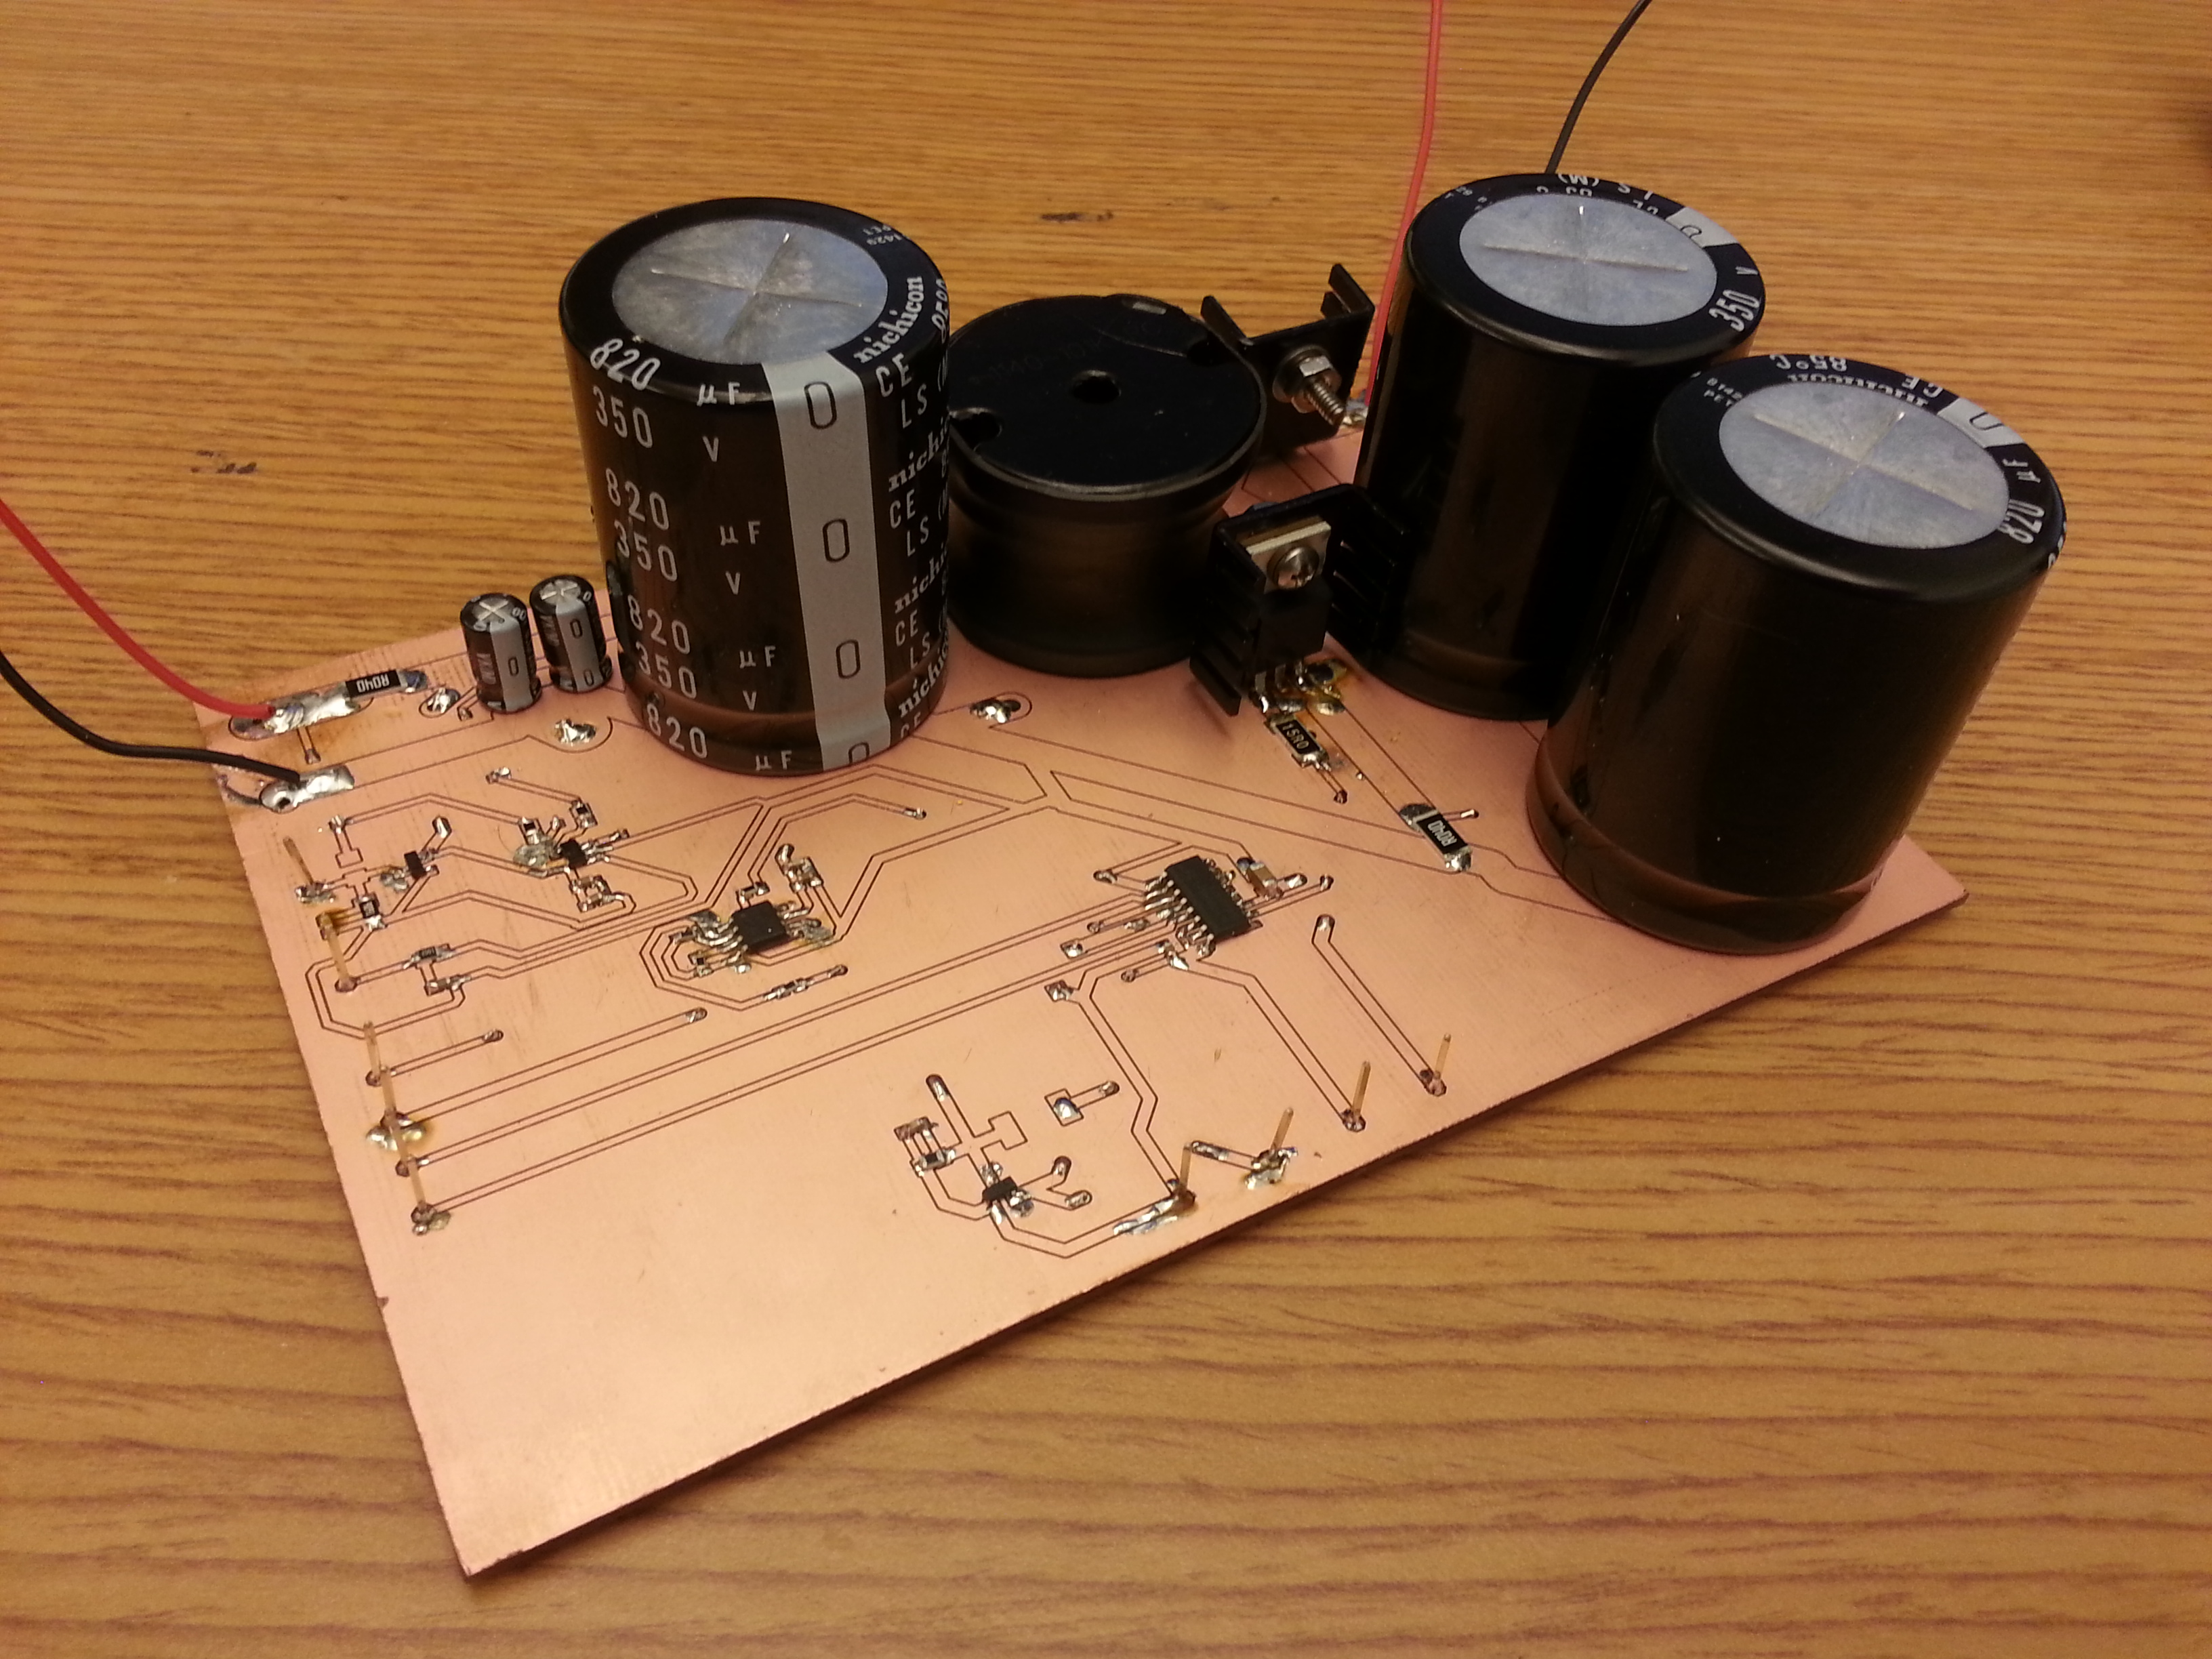
\includegraphics[width = 3.5in]{built_boost.jpg}
\caption{Assembled Boost Circuit}
\label{Built Boost}
\end{figure}

\subsubsection{Boost Converter Efficiency}
Since this boost converter is designed to operate in a solar powered microinverter \todo[inline]{obvious AF by now}, energy conversion efficiency is an important factor \todo[inline]{just say this, maybe in a few more words}. The design aims to mitigate reduced efficiencies which can limit a system's ability to turn energy from the sun into electrical power and waste this energy as heat \todo[inline]{it is clear that inneficiency is wasted as heat}. Ideally, a switching converter will have a 100\% power conversion rate but in practice this is not feasible. Losses due to parasitic resistances and capacitances in circuit components impair the device's efficiency. Rates in the high ninetieth percentile have been achieved in some switching DC/DC converters but efficiencies falling more in the range of 90\% to 70\% are more common and can be deemed acceptable depending on the application. \todo[inline]{you don't need to explain that inefficiency is waste heat, you don't need to spend more than one sentence saying efficiency is important}

There are three main areas of the boost converter that contribute to the most significant power losses \todo[inline]{main and significant, wow, much inefficiency in word use}: the switching transistor, the rectifier diode, and the inductor. \todo[inline]{you dont need to state the role that each compnent plays; if this is not clear by now, you havent done your job. Just say transistor, diode, etc.}The heat generating losses are attributed to periods of conduction and switching with the parasitic conditions. Estimates of the diode losses are calculated earlier to be approximately 2.91W for the boost converter operating at close to the 200W rating. Likewise, the MOSFET losses are calculated to be approximately 1.79W. The series resistance of the inductor does not generate heat to justify heatsinking but still reduces the power as estimated in the following equation.

\begin{equation}
P_L = (I_{in,rms})^2R_L = (5.47A)^2(0.025\Omega) = 0.75W 
\end{equation}


A first order estimate of the boost's efficiency, with the above three loss considerations, is calculated in the following the following equation.

\begin{equation}
\eta_{est} = efficiency_{estimate} = \frac{P_{in} - {(P_{sw}+P_L+P_D)}}{P_{in}} = 97\%
\end{equation}
\todo[inline]{do not write out efficiency_estimate in math mode. Say eta with the appropriate subscript, then explain that variable in text}
This is an optimistic conversion efficiency and does not fully encapsulate an array of other possible factors such as component tolerances and capacitive equivalent series resistances. A deviation of 10\% is a fair engineering estimate on how much this efficiency could drift.

The boost converter circuit prototype allows efficiency testing under the constraints of a laboratory environment. Efficiency is calculated with the relationship shown in the following equation. The operating parameters of the test are: $V_{in} = 12V$,~ $R_{load} = 477.66\Omega$ , $F_{switching} = 50 kHz$. 

\begin{equation}
\eta_{exp} = efficiency_{experimental} = \frac{P_{out}}{P_{in}} = \frac{{V_{out}}^2{R_{load}}}{{V_{in}}{I_{in}}}
\end{equation}
\todo[inline]{same thing here, you do not write out words like this in math mode, use the variable then explain it}

The test uses different PWM duty cycles between 20\% and 73\% to obtain an array of efficiencies as shown in the following equation.

\begin{equation}
Experimental~~ Efficiencies:  ~~  Peak = 85.4\%, ~ Average = 83.84\% 
\end{equation}
\todo[inline]{this is bad style, use the eta variables you defined. Average is denoted with a bar over top, do not write out}

As the testing indicates, the boost converter operates well within the range of standard energy conversion efficiencies. This allows the system to operate without significant undesired heat waste from power drawn from the solar panels.

The boosted output voltage compared to input voltage over different duties is shown in Figure ~\ref{Boost Converter Output Voltage Vs. Duty Cycle} and the voltage gain versus duty is shown in Figure ~\ref{Boost Converter Gain Vs. Duty Cycle}.

\begin{figure}
\centering
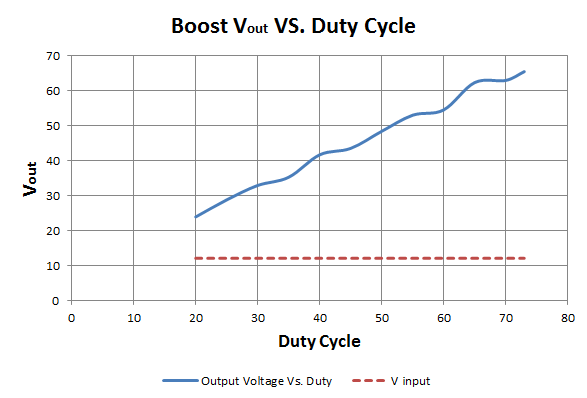
\includegraphics[width = 3.5in]{boost_out_vs_in.PNG}
\caption{Boost Converter Output Voltage Vs. Duty Cycle}
\label{Boost Converter Output Voltage Vs. Duty Cycle}
\end{figure}

\begin{figure}
\centering
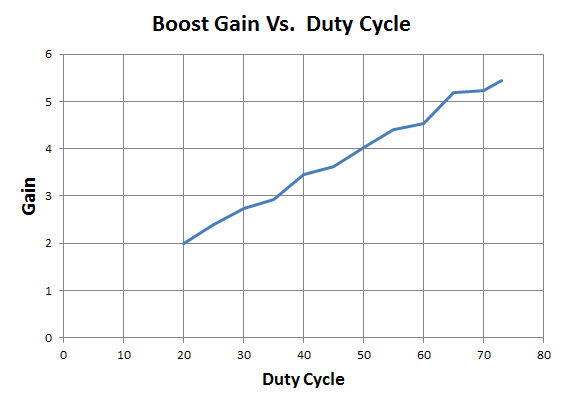
\includegraphics[width = 3.5in]{boost_gain_vs_d.PNG}
\caption{Boost Converter Gain Vs. Duty Cycle}
\label{Boost Converter Gain Vs. Duty Cycle}
\end{figure}



\subsection{H-Bridge}
Arguably, the lynch-pin of any inverter is the H-Bridge circuit. In order to generate a pseudo-sinusoid from a DC source, we must first have the means to switch this DC voltage on and off, and also to drive current bidirectionally. Thus, careful design of the H-Bridge circuit was a critical step in our development.

For a successful H-Bridge design, we needed to consider a number of factors including the speed of switching, deadband, transistor type, transistor gate drivers, thermal analysis, and careful layout due to the speed of the signals involved and the resultant EMI.

After some analysis of the algorithm, further discussed in Section (CITE ME!), we found that the speed of switching with the hybrid algorithm - unlike the switching speed of PWM algorithms which modulate over a fixed carrier frequency - was highly dependent on the width of the tracking band (@todo:Make sure that the tracking band is introduced in BG!). Consequently, there is also a dependence on the resolution of the ADC, and the frequency at which our interrupt is serviced. Through simulations in Matlab we were able to determine that the speed at which the algorithm caused the inverter to switch were well under 100kHz for a 'small-enough' tracking band. 

Because the switching speed is a function of width of the tracking band, sampling rate, and ADC resolution it is by no means a straightforward calculation to determine the frequency of switching. Contrast this to the PWM approach where this determination is trivial. In any case, because the switching speed was tunable by way of modifications to the with of the tracking band, it was decided that it was not necessary to go with more advanced FET technologies like Galium Nitride that are more than capable of switching in the MHz range under full load. 

Shoot through is another important consideration with the H-Bridge circuit, as the possibility of a nearly direct path from power to ground can exist as the circuit switches from outputting +Vdc to -Vdc. To prevent this, a mandatory off time just be implemented in hardware of software. We took the software approach, although the gate drivers we used also implement a minimal deadband in hardware. In the configuration of the PWM driver in our micro controller code, a 20ns headband was implemented, based off of the 60MHz clock.

For the transistors in the H-Bridge, we decided on field effect transistors, (FETs), and in particular the CoolMOS\textsuperscript{TM}
variety built by Infineon. The IPP60 comes in a standard TO-220 package allowing for the use of standard heatsinks, has a Vds max of 650V - about three times what we would need - and a maximum continuous current of 31 Amps. Additionally, these FETs have a very low gate charge (low capacitance, smaller switching losses), low Rds on, and great slew rate. The fact that the drain to source resistance is low helps with our thermal budget, and also means higher efficiency overall. Because of the bipolar switching that the hybrid algorithm called for, we felt that it was wise to over specify our switches. Finally, the freewheeling diode found on many H-Bridge circuits was not needed here since the diode inherent to the construction of the FET was sufficient to handle any expected back currents in our load. 

\subsubsection{Switching Loss and Conduction Loss}
One of the primary factors in the overall efficiency of a modern switching power supply is the switching loss inherent to FET transistor technology, and also the conduction loss associated with Rds on, the resistance of the FET while it is conducting. Switching loss occurs whenever the FET changes state, and can be roughly understood as the net amount of charge it takes to drive the gate of the device. This amount of charge corresponds to a loss of current that could have gone to drive the load in question. This effect can be mitigated in some cases with parallel capacitance at the gate, using `faster' FETs, and choice of the freewheeling diode\cite{switchingLoss}.

The heat sinks in our design are connected to the AC ground. Both the low-side and high-side transistors are insulated from the heat sink with thermal pads and insulating shoulder washers. According to the Transform application note we used as reference during our design, "For the high-side transistor, capacitance between the TO220 tab and the heat sink will add to switching loss, and so a thick and/or low permittivity insulator should be used."\cite{transphorm}

We chose the SI823x family of gate drivers from Silicon Labs, which have a built-in under voltage protection to prevent `nuisance trips' and to add noise margin to our control signal. The gate drivers utilize a bootstrap circuit to operate as both a high-side and low-side driver. 

Because of the relatively high speeds involved with the H-Bridge, careful layout was especially important here. Parasitic capacitance on gate and drain loops are a main cause of overshoot and ringing in the circuit, and thus the total enclosed area between the gate drive and the FETs was kept to the absolute minimum. In order to minimize inductance in the output current path, high current power and ground planes were utilized. Small ferrite beads were used between the gate drive output and the gates of the FETs to reduce ringing cause by coupling of the drain current to the gate drive loop- these were found to be more useful than small resistances which are sometimes used \cite{transphorm}. High voltage SMD ceramic bypass capacitors were placed directly underneath either side of the H-Bridge circuit to minimize the series inductance in the circuit. 
  
\subsection{RLC Output Filter}
The output filter must attenuate high frequency switching noise while passing the 60Hz fundamental intended for standard loads. In a typical PWM design, the driver factor behind the cutoff frequency of the output filter is the carrier frequency of the PWM signal. In most cases, this carrier frequency is invariant, and therefore allows for a relatively straightforward design parameter during the time where components are selected. Of course, THD is also a primary driver of part selection and valuation of the analog components.


In order to ensure that the vector fields on the power plane are such that the hybrid algorithm can ensure forward invariance, and that the solution of the system converges to the tracking band in finite time,  it is necessary that our design adhere to a set of constraints on the RLC filter described in \cite{ricardo}. 

Namely, our filter components must meet the following constraints: first, we must satisfy the condition that $LC\omega^2>1$ - this property ensures our vector fields are oriented correctly throughout the desired trajectory on the VI plane. Second, we have that the capacitor value must be determined by the output voltage amplitude and current amplitude by the relation:$\frac{I_l\omega}{V_c}$ where $I_l$ is the target output current, and $V_c$ is the target output voltage. From this final condition we observe that the value of the capacitance can be driven up by increasing the target current, decreasing the target voltage, or increasing the frequency of operation. 

Let's examine this mathematical condition through the lens of circuit analysis. By inspection, we note the similarity of this condition to the condition for resonance in a series RLC circuit - which is the subject of study in \cite{ricardo}. This condition is given by $\omega_0 = \frac{1}{\sqrt{LC}}$ Taking the square of both sides in the expression, find that $\omega_0^2LC=1$, and we see that the condition on the filter components given states that the resonant frequency of the circuit ought to be greater than unity. If we suppress the variable for capacitance in 
$LC\omega^2>1$ given the condition $C=\frac{I_l\omega}{V_c}$, we obtain:
\begin{equation}
\label{constraint}
L > \frac{V_c}{I_l\omega^2}
\end{equation}

The expression obtained in \ref{constraint} adds a considerable degree of inductance compared to that in a typical PWM inverter. It was considered initially that the quality factor, $Q$ might be at work in the conditions on the filter, but we find that the quality factor for the series RLC filter is given as $Q = \frac{1}{R}\sqrt{\frac{1}{LC}}$, and the analysis in \cite{ricardo} makes no mention of the damping term $R$.

\subsection{Feedback Sense}
The output sensors are an important part for the operation of the inverter since they allow the microcontroller to monitor the output voltages and currents for feedback control. There are eight sensor circuits at the inverter stage and the output filter. The H-bridge portion of the circuit creates the 60 Hz sinusoid signal and this signal requires a variety of sensors considering its oscillatory nature. These signal conditioning circuits are made from passive components and integrated circuit packages to break down high power signals into voltages suitable for microcontroller sampling. \todo[inline]{think about your audience. It is obvious that we are using electronics to build our sensors. Name the circuits, i.e. voltage divider, op amp buffer, differntial amplifier...}
	
After the H-bridge is the output filter which has two AC hot outputs \todo[inline]{do not say AC hot - wht would they be, cold?} for input into the setup transformer \todo[inline]{we have not even mentioned a step-up yet. This is too specific, and it is fairly obvious what our signal chain looks like. We do not need to keep beating a dead horse}. Considering the size of the filter components, they reside on a daughter \todo[inline]{do not say daughter board, choose something else} board separate from the main inverter board. The output power signals have reference jumpers that connect back to the main board after the filtering. \todo[inline]{the point you are trying to get across is very simple, but you use many sentences to say it}The voltages at line and neutral are measured through two voltage dividers. Given their alternating waveforms, the signals will swing below the ground reference potential periodically. Measuring this effect is achieved through the use of a differential amplifier circuit configuration with the scaled AC output voltages used as inputs. The amplifier's input signals are brought up with a DC offset of 1.65V to allow the negative potential swings of the AC signal to be measured. The sine wave crosses the 1.65V raised signal ground threshold 60 times a second during normal operation. These points are considered as zero crossings and a comparator integrated circuit is present for their detection. \todo[inline]{we do not need to say that a sine of frequency 60Hz crosses the zero 60 times in a second. Just state that we have a zero cross detection}The comparator compares the output signal of the differential op-amp to the 1.65V reference and outputs logic high to the microcontroller when the signals match. \todo[inline]{this is not how a schmitt trigger works per-se. Talk about astable feedback}

The input to the H-bridge has a DC voltage resistive divider to monitor its current input levels on the bus. The inverter has two different types of output current sensing at the H-bridge. The first way the AC output current is detected is through the use of low resistance series current shunts. There are two shunt resistors in the low side legs of the H-bridge. The small voltage drops on the 0.04 Ohm resistors are amplified by two differential amplifiers and then sent to the microcontroller. The feedback control software then takes the difference between the two signals in the legs to evaluate the output current. The other current sensor is an inline Hall effect integrated circuit. This IC lies in series with one of the output channels and noninvasively measures a signal linearly proportional to the AC current through the use of the current's magnetic field.

\todo[inline]{this section should be very simple. Talk about the 3 maybe four different types of sensors we have, list where they are and which signals they are monitoring. I helped build the system and I'm having a hard time following. This section needs editing}

\subsection{The Microcontroller}
At the core of our inverter system is the Texas Instruments F28035 `Piccolo' microcontroller. This embedded controller's internal architecture is optimized for the real time control of devices like switching power converters. The Piccolo has a control law co-processor that can operate complex feedback loops without burdening the main processor, freeing the central unit to perform higher level tasks. The device also features versatile pulse width modulation units which are connected to the general purpose outputs for driving the switching power transistors of the boost converter and H-bridge. 

With the myriad of choices available to designers of power systems, the task of selecting a microcontroller for a power conversion system is no easy task. The first step was to survey the current landscape and find some examples of the most popular microcontroller choices currently being used in power applications today. The controllers that we found most frequently were the dsPic family by Microchip, and the Piccolo family by Texas Instruments. The reasons that these two families have found dominance in this field became obvious: they were low cost, had detailed documentation and application notes for power conversion, and support for the 'real-time' control loops that our application demands.

With the choice narrowed down to two families of processors, the task of selecting a processor boiled down to a cost/benefit analysis between the two. Both had similar power consumption, but the TI family of Piccolo controllers came with the option of faster clock speeds, and correspondingly, faster ADC sampling times. Additionally, the resolution of the PWM and ADC modules was more precise than those of comparable Microchip controllers. The final check-box in the TI column was the tight integration of the Piccolo family of controllers into two of the power development boards that we were considering - the Solar Explorer by TI, and a competing offering by Transphorm. 

With code portability from our development kit to a final implementation being of paramount importance, it was decided that we should go with the Piccolo family. In particular, we chose the F28035 for its mix of speed, low-cost, and wide array of digital control capabilities including a unique co-processor feature known as the CLA which enables offloading of many control implementable in assembly. With the integration of this Control Law Accelerator or CLA, we are able to significantly increase the complexity of our algorithms for a given clock speed, while also running multiple state machines and servicing interrupts occuring at multiple frequencies - all while doing it \emph{faster} than would be possible on competing microcontrollers.

Our final hardware design includes anti-aliasing filters for all ADC inputs, and is capable of outputting the values measured at the ADC to DAC pins for debugging purposes. The system uses a 20MHz crystal to set the pace for a phase-locked system clock of 60MHz. External hardware in support of the microcontroller includes voltage protection diodes on GPIO and ADC pins, and isolated communication circuits allowing for the use of USB debugging while protecting against ground loops.

\subsubsection{USB-JTAG interface}
The Piccolo microcontroller supports JTAG boundary scanning for device programming and real time debugging. To connect through the JTAG circuit, several integrated circuit solutions are implemented on our inverter. Programming, or 
`flashing' the micro with code compiled on a workstation necessitates a USB connection to the inverter board. A Future Technology Devices International (FTDI) FT2232D is used to interface a mini USB with the micro by converting the signals to UART. This device also allows the configuration of an EEPROM flash memory array for use with the proprietary Texas Instruments XDS100 debugger use by the Code COmposer Studio IDE. The USB connection provides its own power to the JTAG conversion circuit, so galvanic isolation is used between the USB power supply and that of the main inverter board to prevent ground loops. Digital signals are sent between the two subsystems through a series of digital isolator ICs which use capacitive coupling. A Texas Instruments IC MAX3221 is present as an RS-232 driver/receiver for the serial RX and TX connections between the FTDI chip and the microcontroller.

\section{Photovoltaics}
Photovoltaics, more commonly known as solar panels or solar cells, operate by the principle known as the photoelectric effect. This description of this phenomena won Albert Einstein the Nobel prize in 1905. In this work, he described the quantized energy carried by photons. This energy was found to be $E=hv$, where $h$ is Plancks constant. If we have a pn junction with a thin, heavily doped $n$ region, then a depletion region between the two materials results. This region is observed to extend primarily into the $p$ region with an electric field $E_0$. While we need electrodes to construct a `bulk' solar cell, these electrodes must also allow light to enter the device. This is typically done by forming electrodes into thin finger like structures on the surface. Additionally, antireflective coatings are typically applied to maximize light incident upon the device \cite{materials}.

If we engineer a semiconducting material with a bandgap tuned to the wavelengths of photons emitted from the sun, then the photons strongly interact with the material and are absorbed. The net effect is the emission of electrons which result in an open circuit voltage between the $p$ type and $n$ type materials. If we complete this circuit, we will obviously obtain an electric current which can be used to drive DC loads - this current is known as a photocurrent. 

The engineering of semiconducting materials that can interact with broad ranges of wavelengths is the subject of much research, but is entirely beyond the scope of this report. Rather, we are more concerned with harnessing the direct photocurrents from PV systems readily available today and turning them into alternating currents. 

In order to achieve this goal we must understand the non-linear relationship between the power generated by solar panels and their operating conditions. From an electrical standpoint, a solar cell is best represented through an engineering circuit model of a current source in parallel with a diode. Two significant parasitic resistances are included in series and parallel positions in the model to account for the physical factors of a solar cell. The current source is responsible for the photocurrent $I_{photo}$ generation due to incident light and will feed DC loads present on the cell's terminals. The diode contributes to a dark current $I_{dark}$ which counters the positive photocurrent and accounts for cell loading. The circuit model of an individual solar cell is shown in Figure ~\ref{circuitModel}. \cite{soteris}

\begin{figure}
\centering
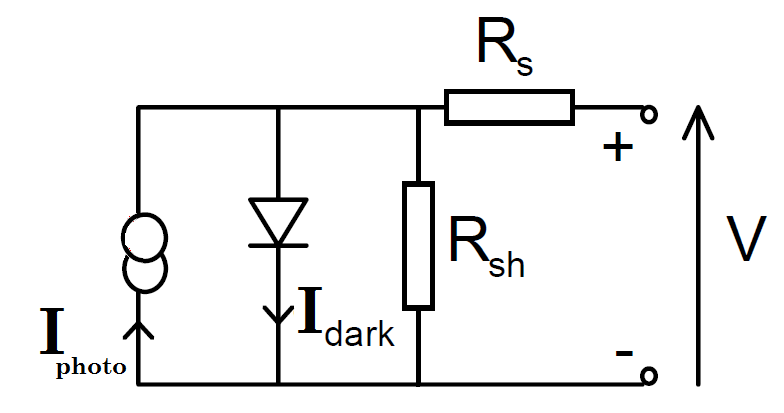
\includegraphics[width = 3.5in]{solar_cell_model.PNG}
\caption{Circuit Model of Solar Cell}
\label{circuitModel}
\end{figure}

Depending on the load, two important parameters can be determined for a solar cell: open circuit voltage $V_{oc}$ and short circuit current $I_{sc}$. The short circuit current will be directly proportional to the intensity of a certain light frequency spectrum for the solar cell and $I_{sc}$ will have a finite maximum value based on the efficiency of the panel. The open circuit voltage occurs when there is no load, massive impedance on the cell terminals, and the dark current through the shunt diode derails any photocurrent. The diode potential drop creates the largest effects on the voltage profile of the solar cell and adds to the non-linearity of the I-V plot for the system as shown in Figure ~\ref{Output Voltage Vs. Current of a Solar Cell}. \cite{soteris}

\begin{figure}
\centering
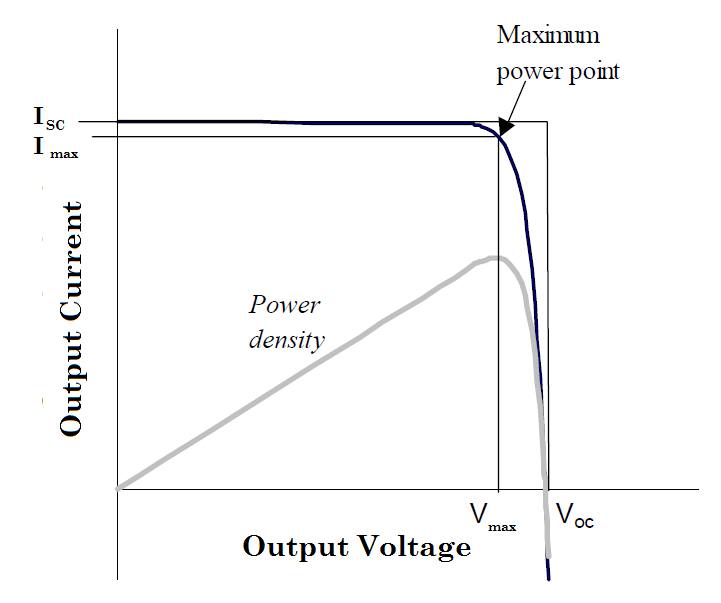
\includegraphics[width = 3.5in]{IV_curve_solar.PNG}
\caption{Output Voltage Vs. Current of a Solar Cell}
\label{Output Voltage Vs. Current of a Solar Cell}
\end{figure}

Drawing maximum power from the solar unit requires a specific DC load which optimizes the product of photocurrent and output terminal voltage to produce the largest possible value. This sourcing configuration is known as the maximum power point that a solar inverter will ideally operate at by varying its impedance. The I-V curve indicates best performance for energy generation when it closely matches a square since this maximizes the power density of the solar cell. Deviations from this optimal shape occur due to the parasitic elements in the engineering model. Output current can be undesirably leeched through the parasitic shunt resistance $R_{sh}$ which is due to current leaks in the semiconductors. The output current is also hindered by the series resistance $R_{s}$ which is present due to contact resistances. Larger $R_{sh}$ and smaller $R_{s}$ values indicate higher quality solar cells. Increased temperatures will also negatively effects the cells by decreasing the maximum possible output voltages.

Solar cells each typically produce under 1V, so multiple cells are be connected in series to create a panel with a useful voltage range. The forward diode in the cell's circuit model has the possibility of drawing current from neighboring cells when they are collected in parallel. Reversed blocking diodes are placed within the panel circuit to mitigate this as the individual cell outputs vary. The complete solar panel features many submodules of solar cells connected to a DC bus network which are then interface with polarized output leads.

\section{The Hybrid Inverter Team Development Board}
The Hybrid Inverter Team's development board aims to be a higher power replacement for TI's Solar Explorer development board with several key changes. Several of the auxiliary modules included with the Solar Explorer that were unnecessary for our design were omitted. The omitted modules included the second microcontroller for solar panel emulation, as well as the SEPIC converter used for battery charging. With the already lofty goal of building a full switch-mode boost and inverter, we felt it would be a great deal of added complexity to build, code, and troubleshoot the SEPIC battery charger for our senior design project. The panel emulator was unnecessary since we would either be running the board from an ATX power supply, or a real solar panel.

Our PCB layouts utilized a four layer design with power and ground planes on the two middle layers. Multiple layers allowed for components to be placed closer together, and achieve a smaller overall form factor while allowing for higher current carrying capabilities. Additionally, we were able to use polygon pours on the central power layers to boost current carrying capacity and aid in the dissipation of heat. Ground plane isolation was used to separate areas with switching power signal and digital logic.

Input and output connection points were placed around the perimeter of the board for easy interfacing with cables. Eagle PCB was utilized for this design and the board house Advanced Circuits was used for board fabrication. Parts were sourced from the Digikey\todo[inline]{just do me a favor and read this}. The top layer of the PCB is shown in Figure ~\ref{PCB top} and the bottom layer in Figure ~\ref{PCB bottom}. The completed circuit board is displayed in Figure ~\ref{hybrid_PCB}.\todo[inline]{really need to work on the wording o this paragraph} 

\begin{figure}
\centering
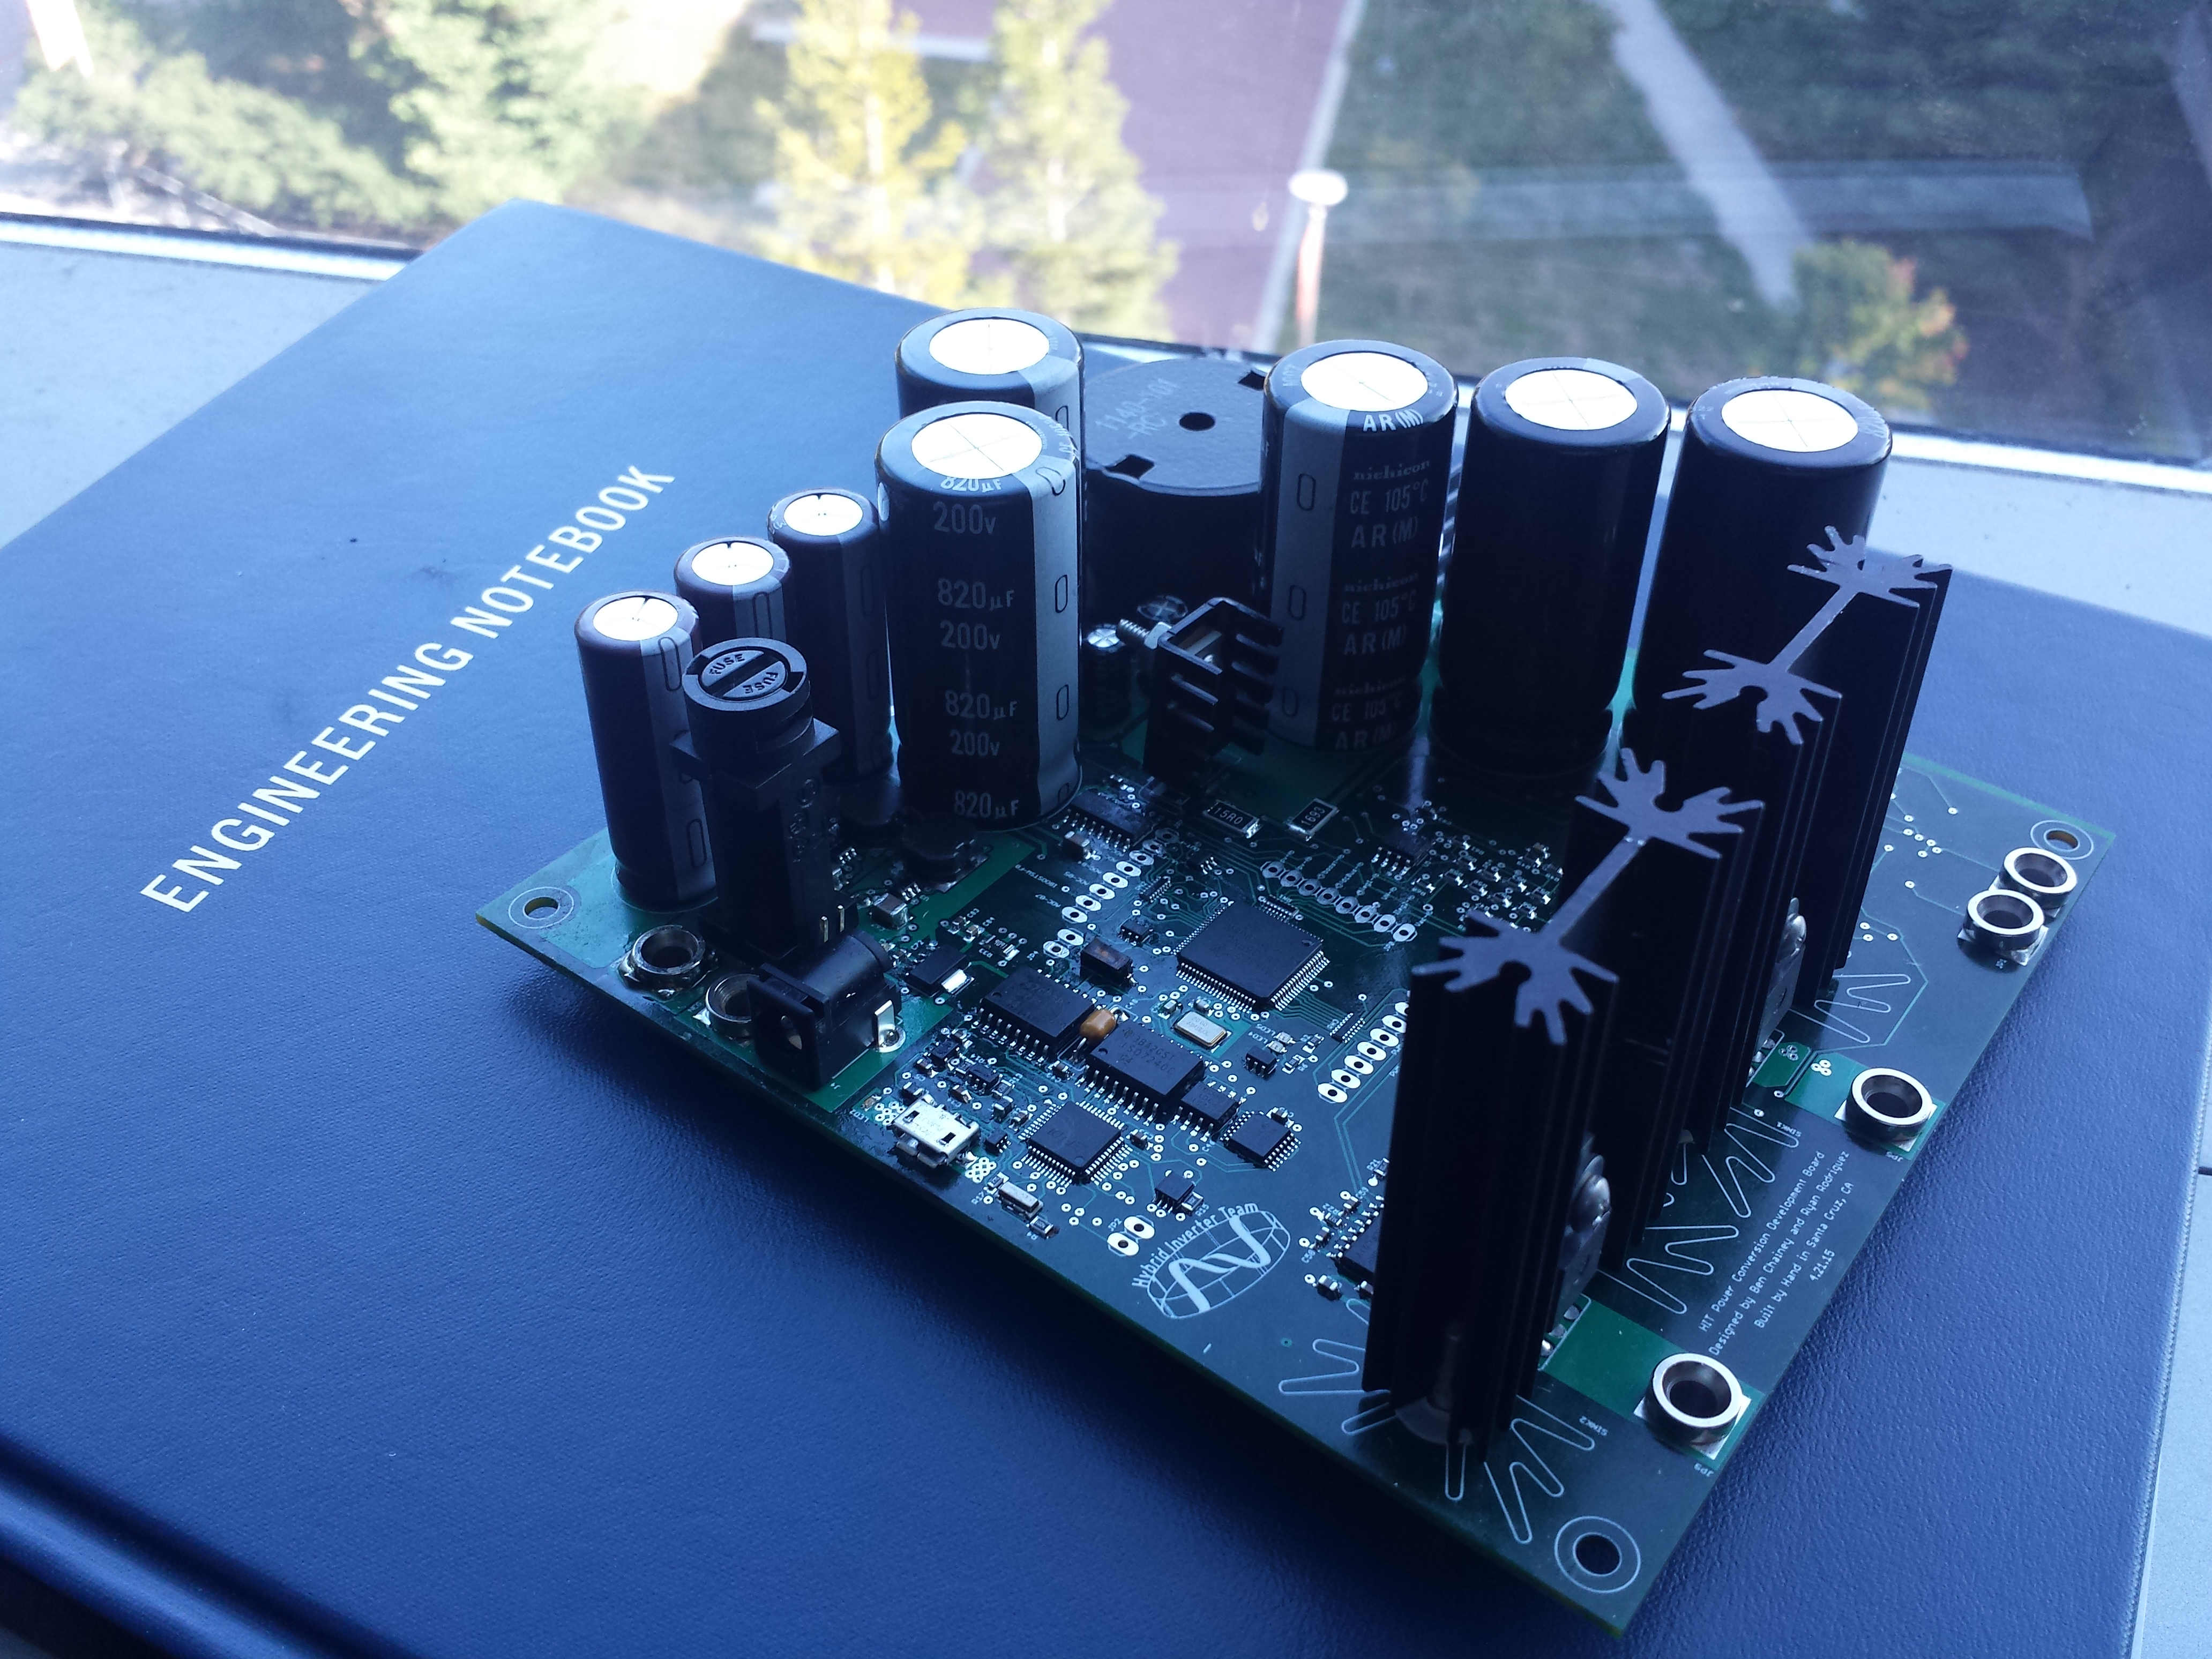
\includegraphics[width = 3.5in]{hitDevBoard}
\caption{The Hybrid Inverter Team's assembled PCB}
\label{The Hybrid Inverter Team's assembled PCB}
\end{figure}


The inverter sits in an enclosure mounted to the back of a solar panel to follow the microinverter topology. The output filter and transformer are constructed using turret board, and is also mounted on the panel mounting system. For testing in outdoor sunlight environments, a wooden stand for the solar panel and inverter system as shown in Figure~\ref{solar stand}.

\begin{figure}
\centering
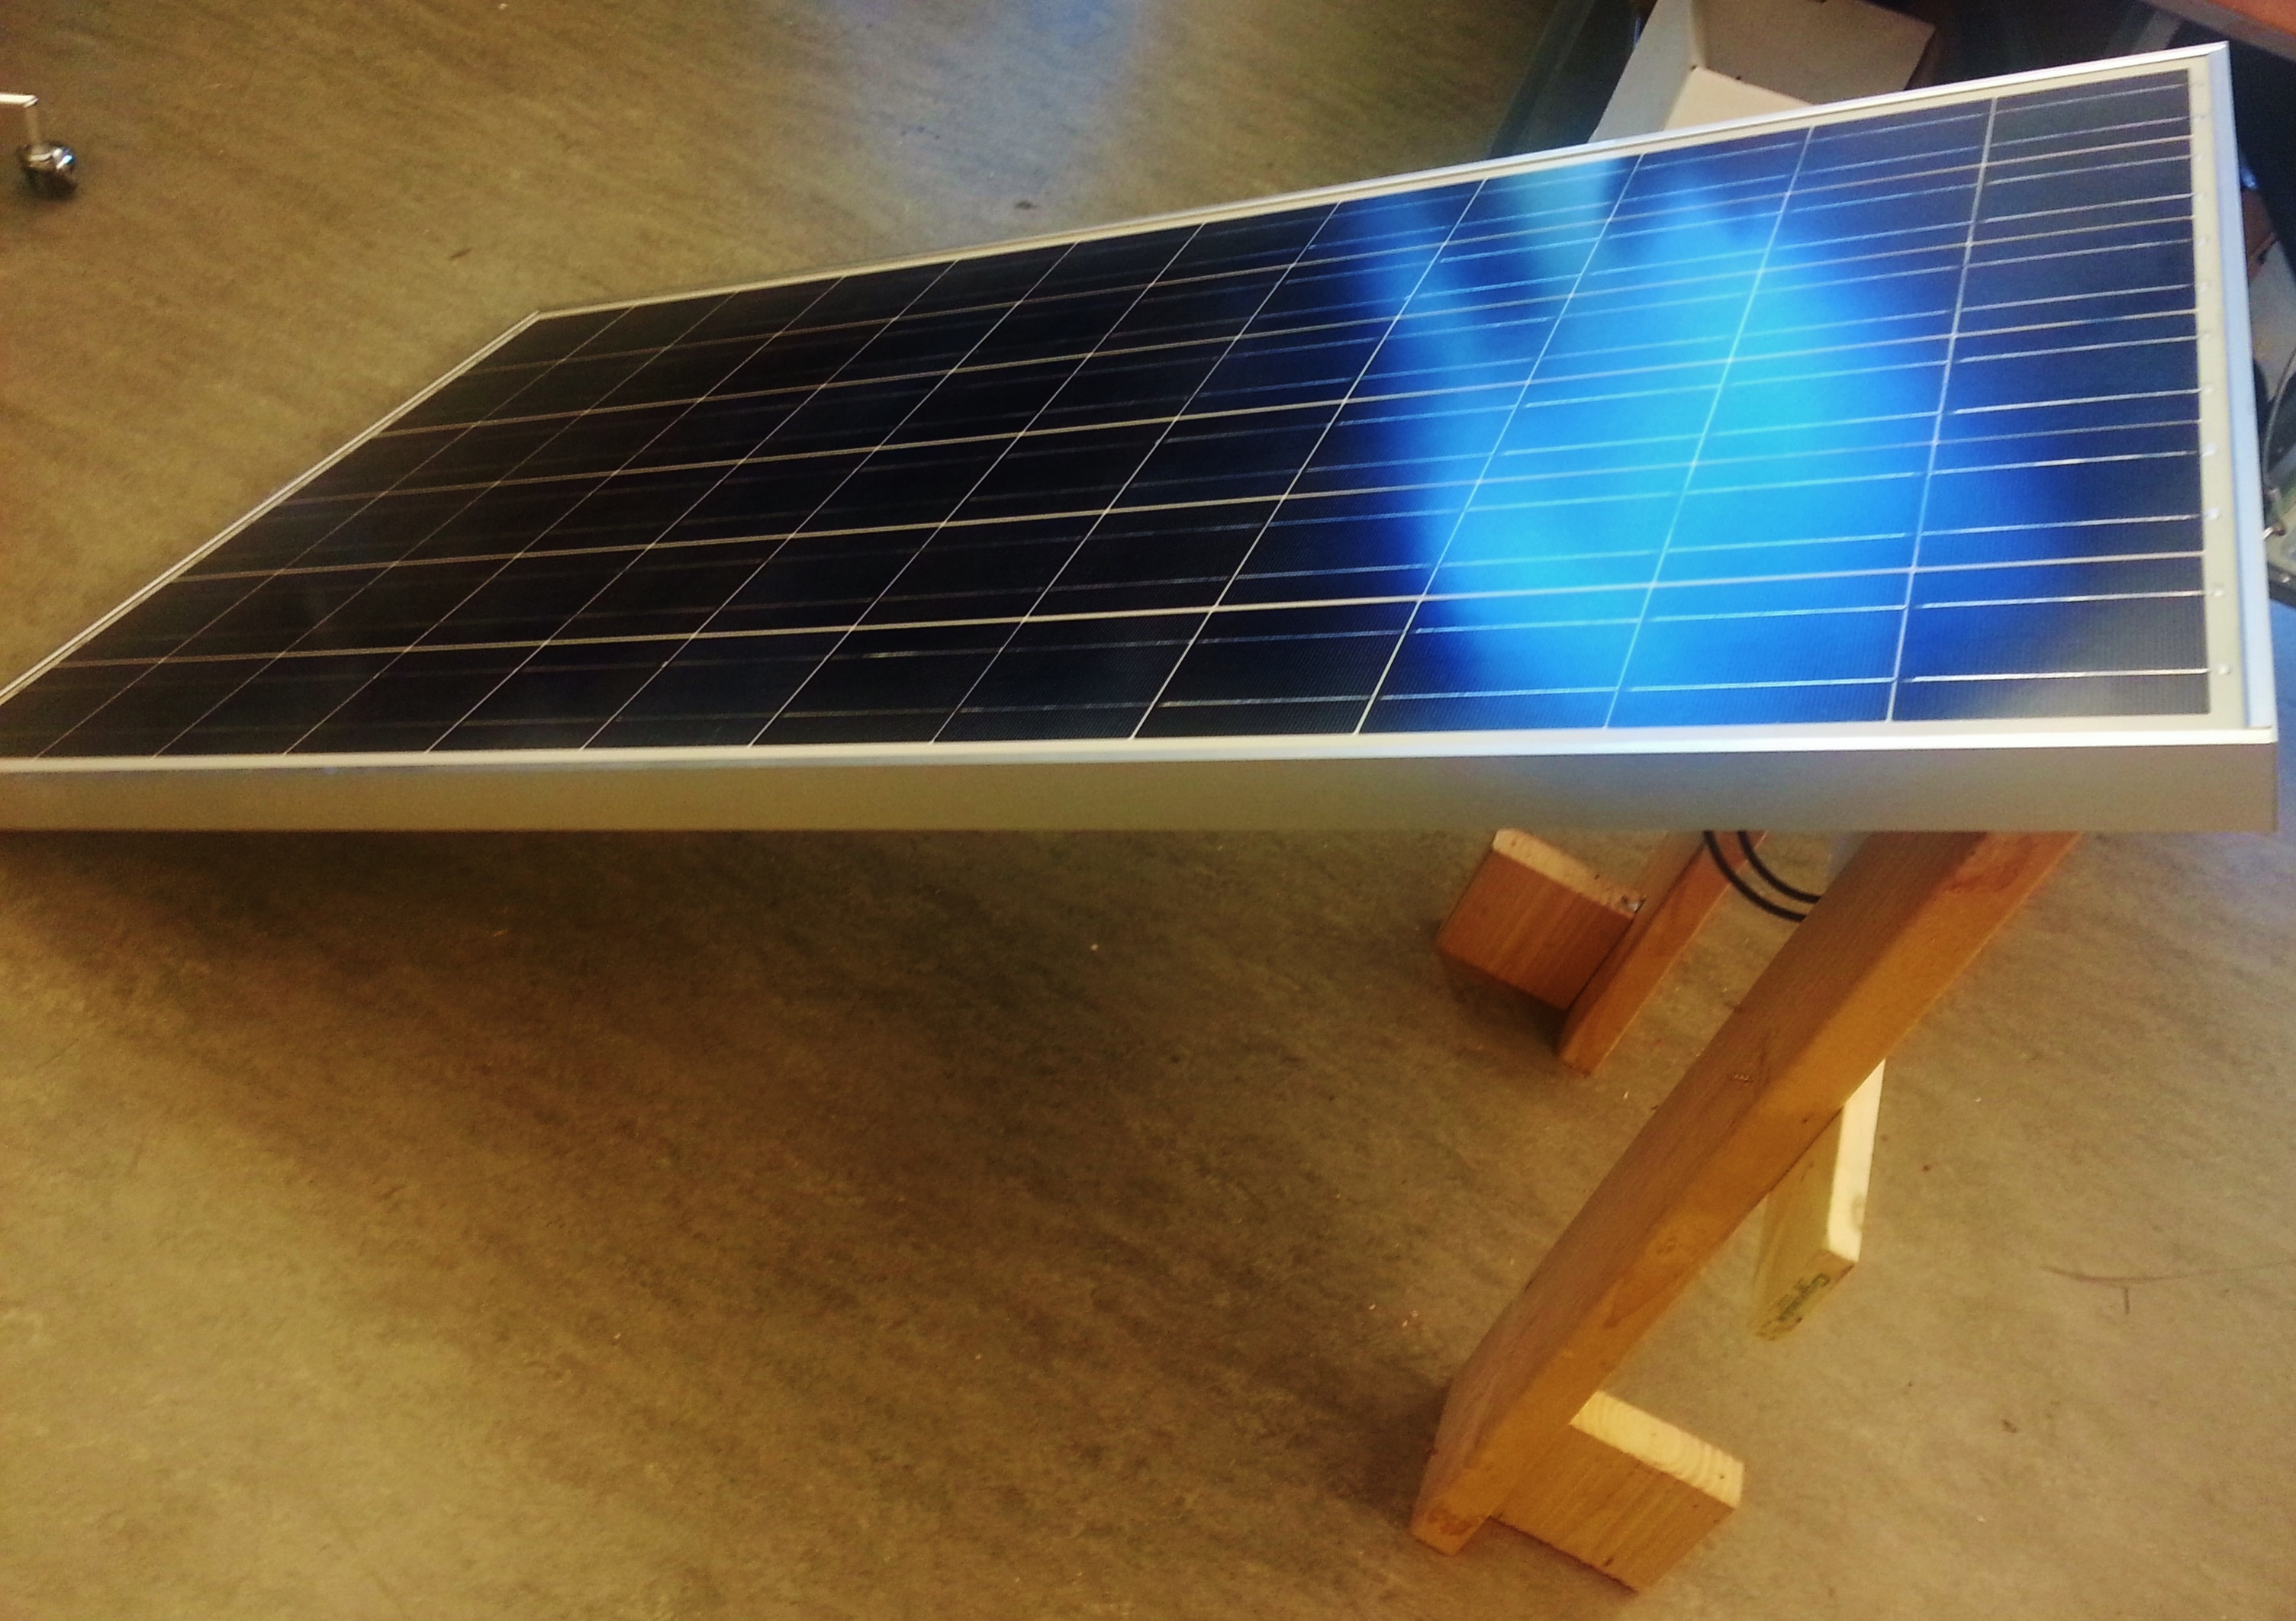
\includegraphics[width = 3.5in]{solar_stand.jpg}
\caption{Solar Panel Stand}
\label{solar stand}
\end{figure}

\subsection{Revision One}
Revision one 
First, we opted to omit the control card socket for a full microcontroller layout with a JTAG interface for debugging. Second, we omitted s

\subsection{Revision Two}


